\section{Maintaining and contributing to a forked repository\label{sec:maintain_repo}}

This section covers the following details

\begin{enumerate}
	\item Checking the status of the forked repository compared to the master repository
	\item Updating forked repository
	\item Making changes to your forked repository
\end{enumerate}

\subsection{Checking the status of the forked repository}

The status of the forked repository as compared to the master repository can be seen on GitHub see Figure~\ref{fig:fork_status})

\begin{figure}[!ht]
	\centering
	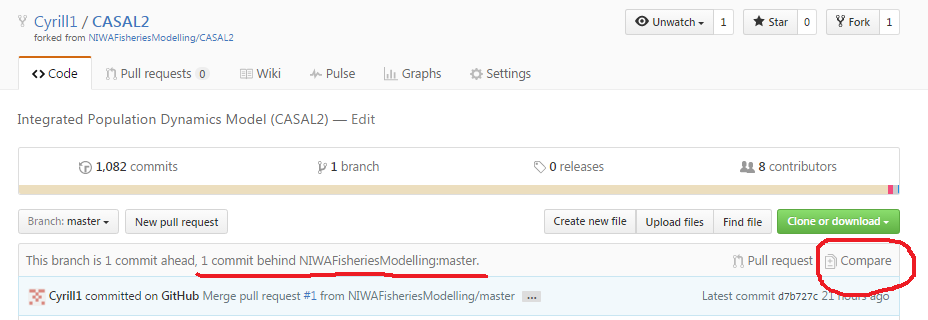
\includegraphics[scale=0.6]{Figures/fork_status.png}
	\caption{Fork status}\label{fig:fork_status}
\end{figure}

This line underlined in blue indicates how many commits have occurred on the forked repo since forking the repo or updating the forked repo. The line underlined in red indicates the commits that have occurred to the master since you forked the repo or last updated it. In the above example, we have made one commit to our forked repo (indicated by the blue) and the forked version is one commit behind the master (indicated by the red). 



\subsection{Updating the forked repository to incorporate changes committed to the master}

To update your forked repository to be the same as the master, click the `compare' button (circled in red on the right of Figure~\ref{fig:fork_status}). This will bring up a page that will tell you of the changes that have occurred to the master repository. 
\clearpage
\begin{figure}[!ht]
	\centering
	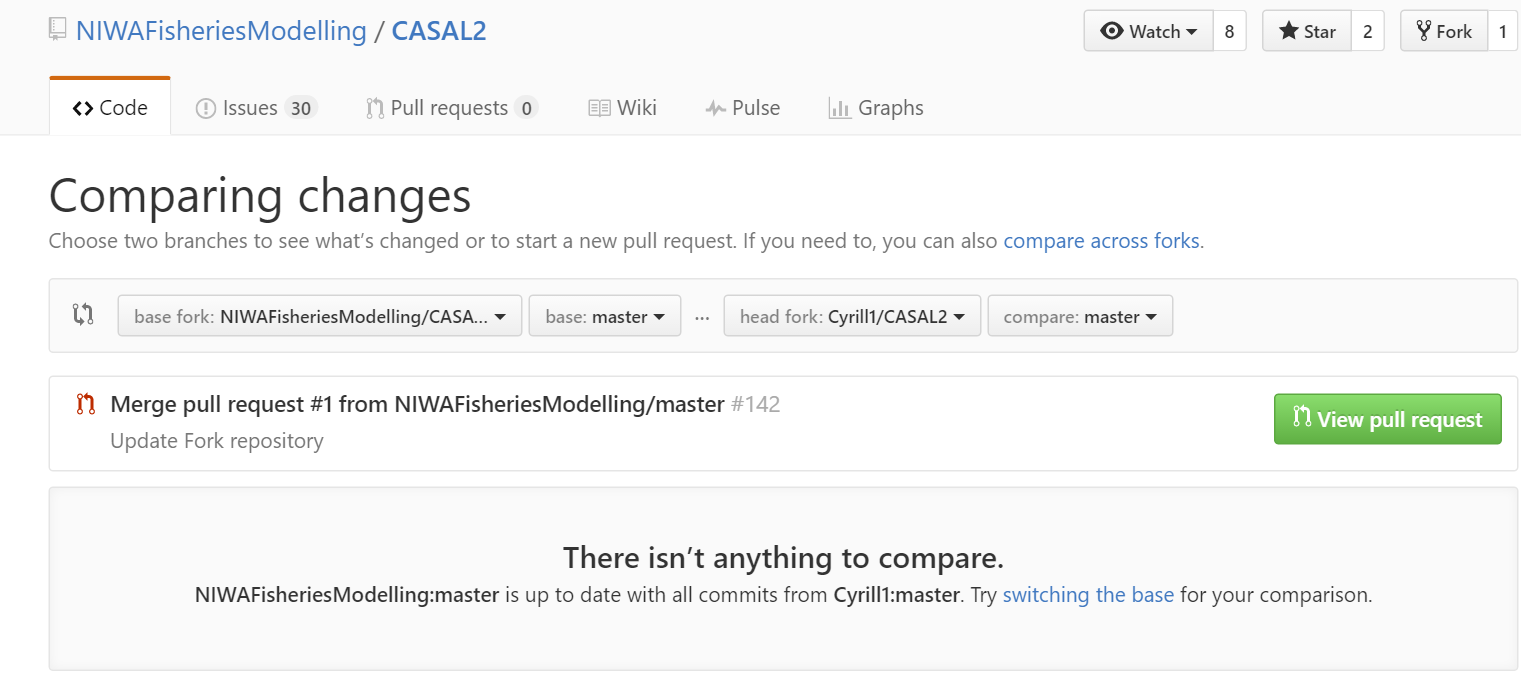
\includegraphics[scale=0.6]{Figures/Compare_fork3.png}
	\caption{}\label{fig:fork_compare1}
\end{figure}

If the following figure appears (Figure~\ref{fig:fork_compare1}) telling you "there isn't anything to compare" click on the \texttt{switching the base} underlined in red.
\raggedbottom
\begin{figure}[!ht]
	\centering
	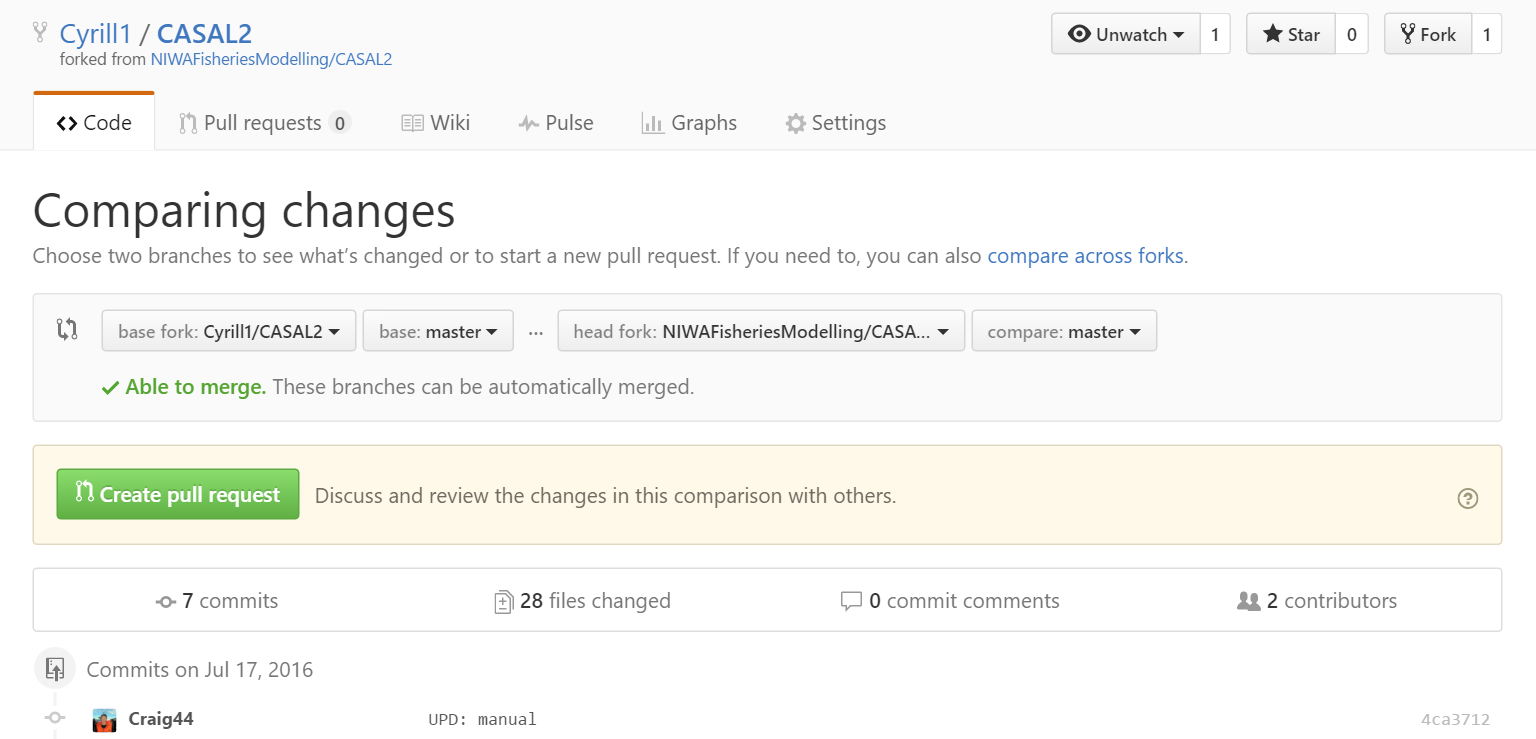
\includegraphics[scale=0.6]{Figures/Compare_fork4.png}
	\caption{}\label{fig:fork_compare2}
\end{figure}

You can see that there are 7 commits and 28 files changed on the master that we want to merge into our forked repo. You can see that there is now a "create pull request" and a green message saying "Able to merge". This indicates you will be able to update your forked repo with ease. Click on the "create pull request" button. This will open a git pull request (Figure~\ref{fig:fork_compare3}) we suggest adding a nice title for the merge like "Updating Craig's Forked Repository" 
\clearpage
\begin{figure}[!ht]
	\centering
	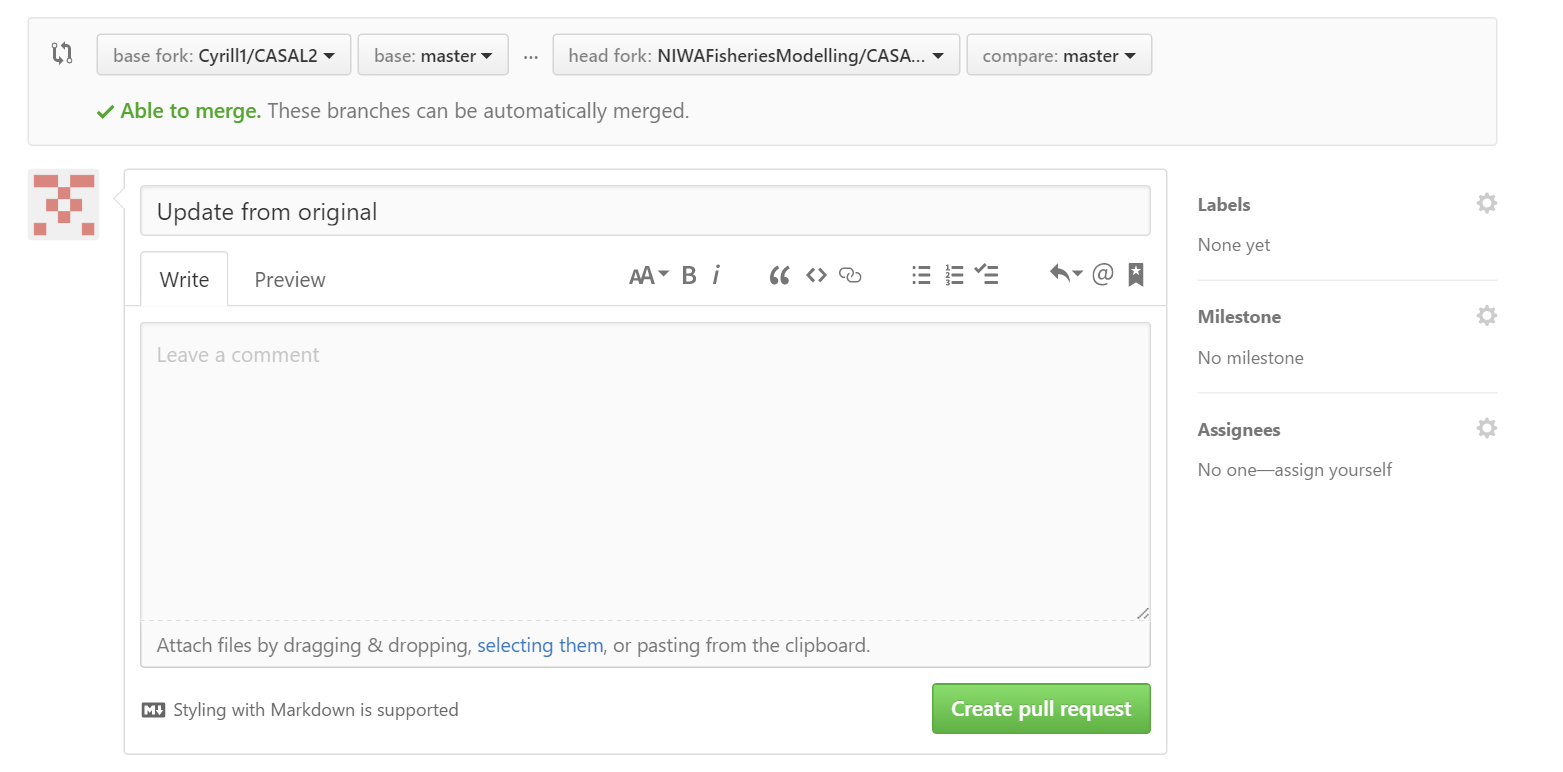
\includegraphics[scale=0.6]{Figures/Compare_fork5.png}
	\caption{}\label{fig:fork_compare3}
\end{figure}

Once you write a reasonable title and click create pull request if there are no conflicts, you can merge the changes from the master into your forked repo by clicking "merge pull request" form Figure~\ref{fig:fork_compare4}.

\begin{figure}[!ht]
	\centering
	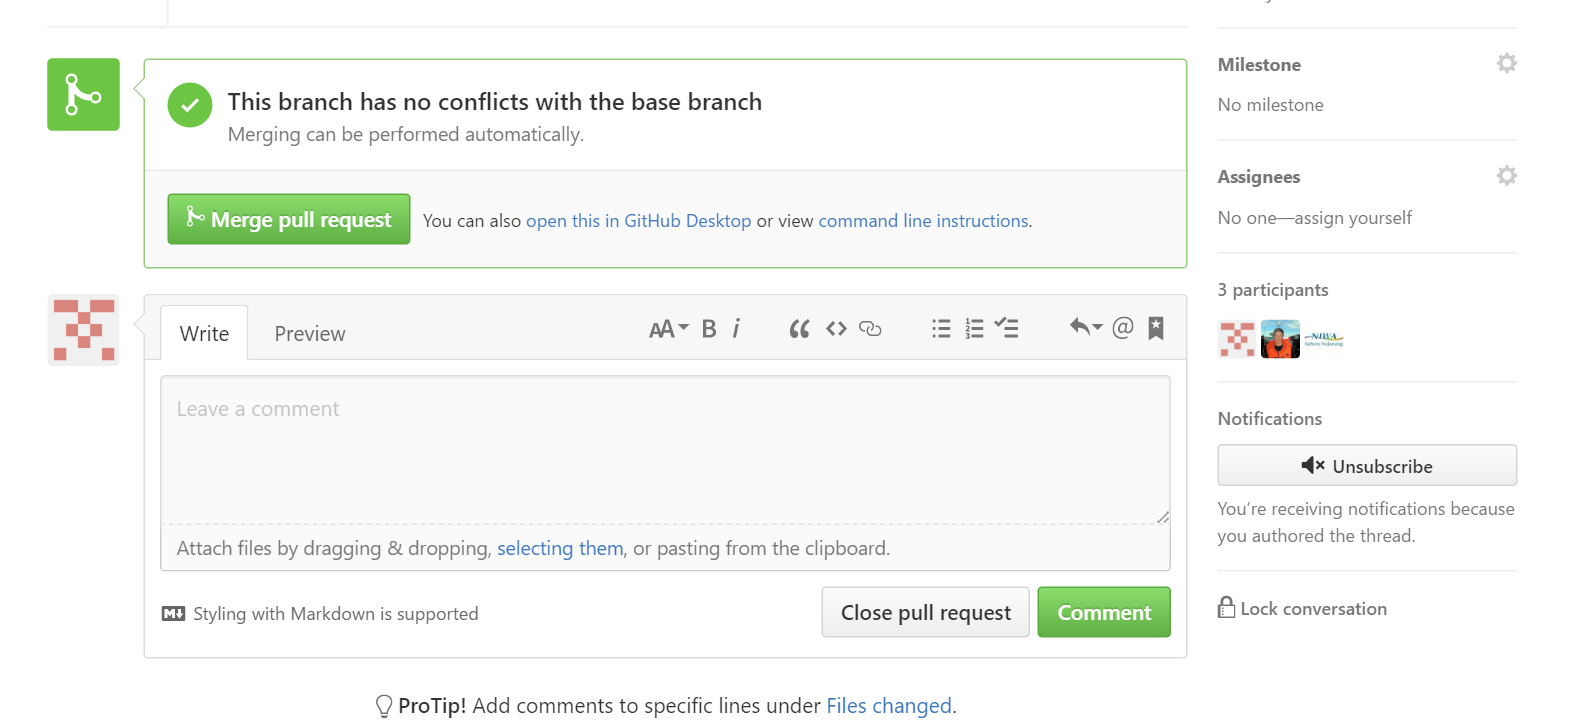
\includegraphics[scale=0.6]{Figures/Compare_fork6.png}
	\caption{}\label{fig:fork_compare4}
\end{figure}
\clearpage
Once you have clicked that you will be told that the merge was a success as shown in Figure~\ref{fig:fork_compare5}.
\begin{figure}[!ht]
	\centering
	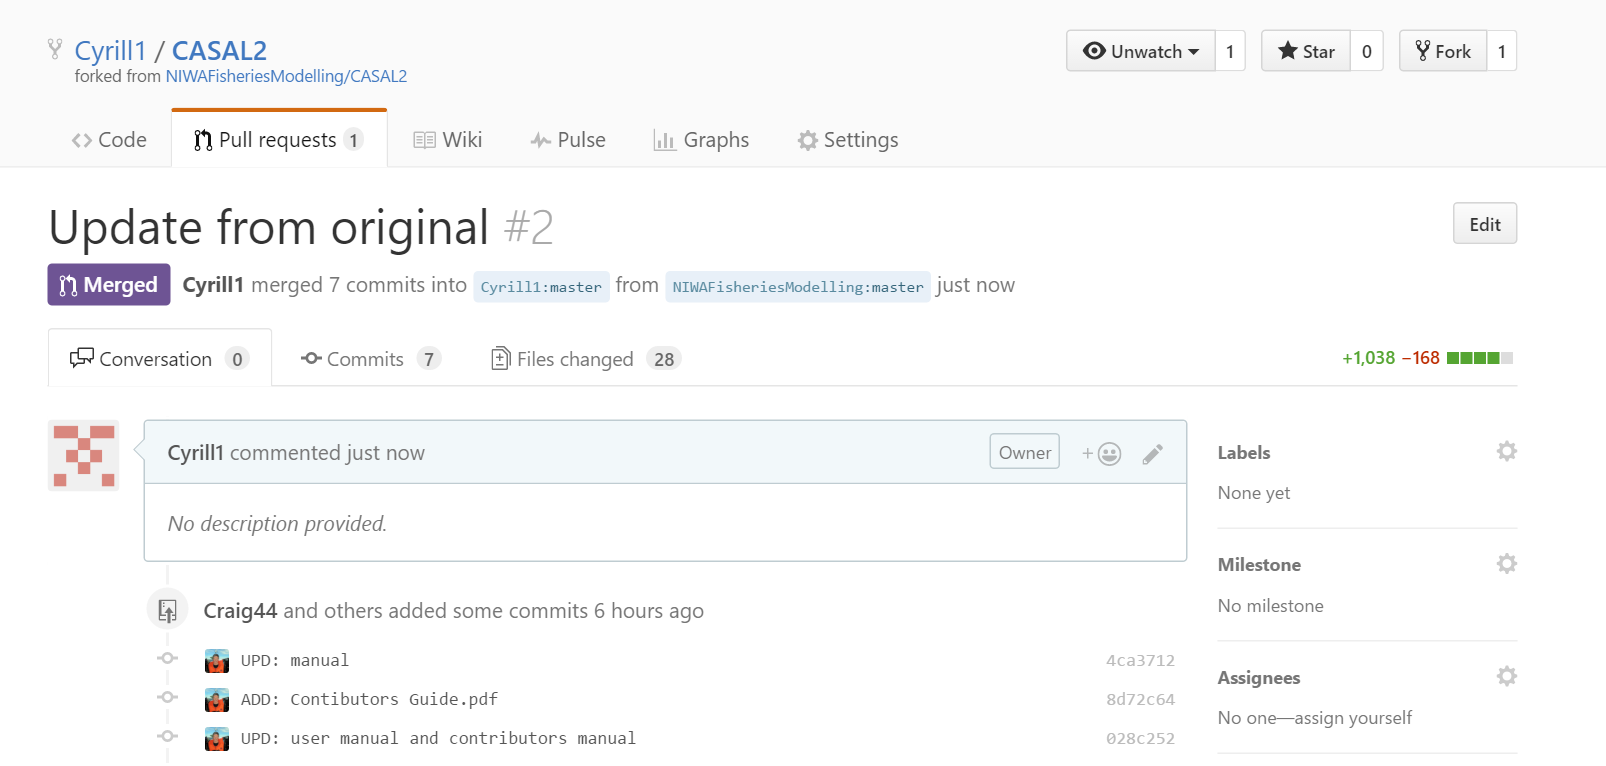
\includegraphics[scale=0.6]{Figures/Compare_fork7.png}
	\caption{}\label{fig:fork_compare5}
\end{figure}

Now you have successfully updated your remote forked repository. To incorporate these changes into your local repository on your computer you just need to do a pull and the code changes should be incorporated in your next build.
